% !TeX root = spherical_harmonics.tex
% !TeX spellcheck = de_DE
Auch wenn wir eingangs in unserem Kurs so sehr über Basen geschimpft haben\footnote{Wir wollen keine Namen nennen, aber Johannes war besonders hartnäckig...}, so ist uns natürlich bewusst, dass gerade für effiziente Berechnungen eine Basis praktisch immer gewählt wird. Welche Basis man wählt, ist dabei von großer Bedeutung: Andrea hat in ihrer Doktor-Arbeit eine bestimmte Berechnung, welche z.B. zur Modellierung von Luftbewegung millionenfach wiederholt genutzt werden soll, um den Faktor 1000 verschnellern können, und das nur durch geschickte Basiswahl. 

\begin{remark}
	Meistens ist eine Basis geschickt gewählt, wenn sie orthogonal bzgl. eines zu Problem passenden Skalarprodukts ist. Nun gibt es aber viele Skalarprodukte, die man wählen kann, die durchaus auch unterschiedliches Verständnis von Orthogonalität festlegen.
\end{remark}
Schauen wir uns einmal einige Beispiele für mögliche Skalarprodukte auf dem Raum der Polynome an:
\begin{example}
	Sei $B$ die Kugel in $\IR^3$ mit Radius 1. Dann ist mit
	\begin{align*}
		\braket{f,g}_B :&= \int_B f g \dd B
	\end{align*}
	ein Skalarprodukt auf dem Raum der Polynome gegeben.
\end{example}

\begin{example}
	Sei $Z$ ein Zylinder in $\IR^3$, z.B. mit Radius und Höhe 1. Dann ist mit 
	\begin{align*}
		\braket{f,g}_Z :&= \int_Z f g \dd Z
	\end{align*}
	ein Skalarprodukt auf dem Raum der Polynome gegeben.
\end{example}

\begin{example}
	Sei $K$ ein Kegelstumpf in $\IR^3$, z.B. mit oberen Radius und Höhe 1 sowie unterem Radius $\frac{1}{2}$. Dann ist mit 
	\begin{align*}
		\braket{f,g}_K :&= \int_K f g \dd K
	\end{align*}
	ein Skalarprodukt auf dem Raum der Polynome gegeben.
\end{example}

\begin{example}
	Sei $Q$ ein Quader in $\IR^3$, z.B. mit den Kantenlängen 1, 2, und 3. Dann ist mit 
	\begin{align*}
		\braket{f,g}_Q :&= \int_Q f g \dd Q
	\end{align*}
	ein Skalarprodukt auf dem Raum der Polynome gegeben.
\end{example}

\begin{centralquestion}
Wäre es nicht praktisch, eine Basis zu finden, die für möglichst viele Skalarprodukte orthogonal ist? Wie würdet ihr mit dem neu erworbenen Wissen nach solch einer Basis suchen? Diskutiert über eure Ansätze und versucht einen Algorithmus zu entwickeln, der eine möglichst allgemein einsetzbare Basis konstruiert.
\end{centralquestion}

\pagebreak
\begin{remark}
Am besten wählt man eine Basis, die möglichst gut an das gegebene Problem angepasst ist, doch was genau heißt das? Für die Auswahl an Problemen in diesem Kurs haben wir festgelegt, dass es sich um Probleme in unserer physikalischen Welt handeln soll. Wir haben uns bereits angeschaut, wie sich diese Einschränkung mathematisch äußert: Alles was wir messen wollen, muss natürlich, also $O_3$-verträglich sein. Wir haben uns auch schon mit der Darstellungstheorie von $O_3$ und einigen ihrer Untergruppen beschäftigt und festgestellt, dass $O_3$ den Raum der Polynome (oder äquivalent: den Raum der symmetrischen Tensoren) in irreduzible Unterräume zerlegt. 
\end{remark}
\begin{remark}
Die irreduziblen Unterräume sind besonders: Wir haben bereits sehr gut verstanden, dass sie immer (also für jedes $O_3$-verträgliche Skalarprodukt) senkrecht zueinander stehen und dass lineare Abbildungen zwischen zwei irreduziblen Unterräumen entweder 0 oder ein Vielfaches der Identität sein können. Wenn man also eine lineare Wirkung berechnen möchte, erspart man sich durch die Zerlegung in irreduzible Unterräume einiges an Arbeit: Alles, was zu bestimmen ist, sind die Konstanten, mit der die Identität zwischen zwei zueinander isomorphen irreduziblen Unterräumen koppeln.
\end{remark}
\begin{remark}
Im übrigen: Für bilineare Abbildungen ist es etwas komplizierter, aber die grundsätzliche Aussage bleibt bestehen: Alle Abbildungen sind entweder 0 oder Vielfache einer Identität (auch dann wenn die Identität etwas komplizierter zu berechnen ist).
\end{remark}
\begin{remark}
 All dies legt nahe, dass eine Basiswahl, die an die irreduziblen Unterräume angepasst ist, praktisch immer eine gute Idee ist. Jetzt sind diese irreduziblen Unterräume aber allermeistens nicht ein-dimensional, wie sucht man sich nun eine möglichst kanonische Basis aus? 
\end{remark}
\begin{remark}
	\label{rem:einbettung_in_physik}
 Hinzu kommt, dass die irreduziblen Unterräume zwar für ganz $O_3$ irreduzibel sind, aber es gibt einige Probleme in der Physik, die eher einer Einbettung von $O_2$ in $O_3$ gleichen, z.B. (Teilchen-) Kollision an einer Wand, eine ausgezeichnete Richtung haben, z.B. die Bewegung von geladenen Teilchen durch einen Kondensator, oder rotierende Systeme beschreiben (Einbettung von $SO_2$ in $O_3$.
\end{remark}

 \begin{remark}
 	Idealerweise ist unsere Basis auch für solche Fälle ausgelegt. Es stellt sich heraus, dass beide Probleme gleichzeitig gelöst werden können.
 \end{remark}
 \begin{definition}[Konstruktion der $\Gae\jae\el\soft\fae\aaa\en\dae$-$\Zae\jae\tae\el\iii\en$-$\Bae\aaa\sae\iue$ (Gelfand\footnote{Israel Gelfand, $\I\sae\rae\aaa\iii\el\soft$ $\Em\ooo\iii\ssae\jae\jae\wae\iii\tschae$ $\Gae\jae\el\soft\fae\aaa\en\dae$ (1913--2009), sowjetischer Mathematiker}-Zetlin\footnote{Michael Zetlin, $\Em\iii\xa\aaa\iii\el$ $\El\soft\wae\ooo\wae\iii\tschae$ $\Zae\jae\tae\el\iii\en$ (1924--1966), russ. Mathematiker und Physiker; Der Name wird leider auf viele verschiedene Weisen transkribiert, u.A. eben Zetlin (meist im dt. Sprachraum), aber auch Tsetlin (engl. Sprachraum), Zeitlin, Tseitlin, Ceitlin}-Basis]
 	\label{def:konstruktion_gz_basis}
	Sei $G$ eine Gruppe mit halb-einfacher Darstellung auf einem Vektorraum $V$ und $U^i_0$ einer der irreduziblen Unterräume von $V$. Für diesen Unterraum wird dessen \emph{Gelfand-Zetlin-Basis} wie folgt konstruiert:
	\begin{enumerate}[label={\arabic*.)}]
		\item Setze das Level $l=0, H_0 = G$
		\item Bestimme für jeden Unterraum $U_l^i$: \label{def:gz_it_anfang}
		\begin{enumerate}
			\item Berechne $\dim{U_l^i}$
			\item Ist $U_l^i$ 1-dimensional? Dann wähle einen Vektor aus $U_l^i$ als einen der Basisvektoren von $U^1_0$.
			\item Ist $U_l^i$ $>1$-dimensional? Dann merke dir $U_l^i$ für den nächsten Schritt.
		\end{enumerate}
		\item Wähle geschickt eine möglichst große Untergruppe $H_{l+1}$ von $H_{l}$, sodass jeder Unterraum $U_l^i$ mit $\dim{U_l^i}>1$ in für $H_{l+1}$ irreduzible Unterräume  zerfällt. Dabei müssen alle Unterräume, die von einem gemeinsamen $U_l^i$ stammen, paarweise nicht isomorph sein (Klappt dies nicht, ist entweder eine andere Untergruppe zu finden, oder es gibt keine Gelfand-Zetlin-Basis). \label{def:gz_it_ugschritt}
		\item Nummeriere die Unterräume des nächst-höheren Levels: Nenne alle für $H_{l+1}$ irreduziblen Unterräume $U_{l+1}^{1}, \cdots, U_{l+1}^{k}$, inklusive der bereits für $H_l$ 1-dimensionalen Unterräume.
		\item Erhöhe das Level um 1: $l++$. \label{def:gz_it_ende}
		\item Wiederhole die Schritte \ref{def:gz_it_anfang} bis \ref{def:gz_it_ende}, bis alle Unterräume vom nächst-höheren Level 1-dimensional sind.
		\item $l_{\text{max}} = l$
		\end{enumerate}
\end{definition}
\begin{remark}
	Formal betrachtet, brauchen die 1-dimensionalen Untergruppen nicht für Schritt \ref{def:gz_it_ugschritt} ausgeschlossen werden. Sie werden für jede Untergruppe 1-dimensional bleiben und sich nicht weiter ändern, entsprechend braucht man sie für die weiteren Schritte auch nicht zu berücksichtigen.
\end{remark}
\begin{definition}[$\Gae\jae\el\soft\fae\aaa\en\dae$-$\Zae\jae\tae\el\iii\en$-$\Dae\jae\rae\jae\wae\ooo$ (Gelfand-Zetlin-Baum)]
	Mit der Konstruktion nach \ref{def:konstruktion_gz_basis} bauen wir einen Baum mit $l_{\text{max}}$ Leveln. Der Stammknoten ist $U_0^i$, die Blätter sind alle gefundenen 1-dimensionale Unterräume. Die Knoten zwischen dem Stammknoten und den Blättern entsprechen den irreduziblen Unterräumen der jeweiligen Level, die Kanten verbinden einen irreduziblen Unterraum $U$ eines Levels mit allen irreduziblen Unterräumen des nächst-höheren Levels, die aus $U$ im Schritt \ref{def:gz_it_ugschritt} herauskommen. Eindimensionale Unterräume, die bereits in kleineren Leveln auftreten, werden hier als Knoten auf jedem höheren Level wiederholt bis zum maximalen Level.
	Diesen Baum nennen wir \emph{Gelfand-Zetlin-Baum}. Er kann z.B. wie folgt aussehen:
	\begin{align*}
		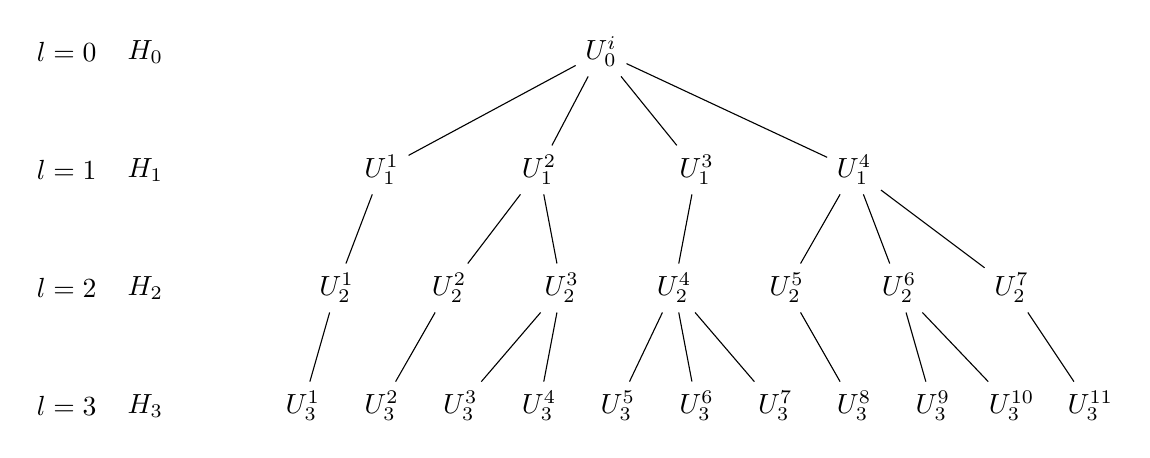
\begin{tikzpicture}[baseline={([yshift=-2ex]current bounding box.center)}]
			\foreach\x  in {1,2,...,11}{
				\node (u3\x) at (\x,-4.5){$U_3^{\x}$};
			}
%			\foreach\x  in {1,2,3.5,6,8,9.5,11}{
%				\node (u2\x) at (\x,-3){$U_2^{\x}$};
%			}
			\foreach\x [evaluate=\x as \y using {\x*10/7}] in {1,2,...,7}{
				\node (u2\x) at (\y,-3){$U_2^{\x}$};
			}
%			\foreach\x  in {1,2.75,6,9.5}{
%				\node (u1\x) at (\x,-1.5){$U_1^{\x}$};
%			}
			\foreach\x [evaluate=\x as \y using {\x*10/5}] in {1,2,...,4}{
				\node (u1\x) at (\y,-1.5){$U_1^{\x}$};
			}
			\node (u0) at (4.7875,0){$U_0^i$};
			\foreach\x in {1,2,...,4}{
				\draw[] (u0) to (u1\x);
			}
			\draw[] (u11) to (u21);
			\draw[] (u12) to (u22);
			\draw[] (u12) to (u23);
			\draw[] (u13) to (u24);
			\draw[] (u14) to (u25);
			\draw[] (u14) to (u26);
			\draw[] (u14) to (u27);
			\draw[] (u21) to (u31);
			\draw[] (u22) to (u32);
			\draw[] (u23) to (u33);
			\draw[] (u23) to (u34);
			\draw[] (u24) to (u35);
			\draw[] (u24) to (u36);
			\draw[] (u24) to (u37);
			\draw[] (u25) to (u38);
			\draw[] (u26) to (u39);
			\draw[] (u26) to (u310);
			\draw[] (u27) to (u311);
			\foreach\x [evaluate=\x as \y using {-\x*1.5}] in {0,1,...,3}{
				\node (l\x) at (-2,\y){$l=\x$};
				\node (h\x) at (-1,\y){$H_{\x}$};
			}
		\end{tikzpicture}
	\end{align*}
	In einem Gelfand-Zetlin-Baum sind alle Darstellungen paarweise ungleich. Es kann aber auftreten, dass manche Darstellungen isomorph zueinander sind (wobei die Kinder eines Knotens niemals isomorph zueinander sein dürfen).
\end{definition}
\begin{remark}
		Die Wahl der Untergruppen-Kette $H_1\cdots H_{l_{\text{max}}}$ ist hier spielentscheidend und keinesfalls eindeutig. Aus diesem Grund gehört zu einer vollständigen Anweisung \enquote{Wähle eine Gelfand-Zetlin-Basis für $G$ auf $V$} auch die Angabe der Untergruppenkette $H_1\cdots H_{l_{\text{max}}}$.
\end{remark}
\begin{remark}
	Auch wenn die Konstruktion einer Gelfand-Zetlin-Basis klappt, hat man nicht unbedingt etwas gewonnen. Wenn man dazu besonders exotische Untergruppen benutzen muss, bringt einem die Gelfand-Zetlin-Basis in der Anwendung nicht besonders viel. Eigentlich möchte man sich erst für eine Untergruppenkette $H_0\cdots H_{l_{\text{max}}}$ entscheiden und dann schauen, ob die Konstruktion funktioniert.
\end{remark}
\begin{definition}[$\Gae\jae\el\soft\fae\aaa\en\dae$-$\Zae\jae\tae\el\iii\en$-$\Bae\aaa\sae\aaa$]
	\label{def:gz_basis}
	Sei $G$ eine Gruppe mit Darstellung auf einem Vektorraum $V$ und $G$ zerlege $V$ in seine irreduziblen Unterräume $U^1_0,\cdots U^k_0$. Wähle außerdem eine Untergruppenkette $H_1 \gneq\cdots\gneq H_{l_{\text{max}}}$. Für jeden dieser Unterräume wird nun einzeln eine Basis $\mathcal{B}$ konstruiert nach \ref{def:konstruktion_gz_basis}. $\mathcal{B}$ heißt dann \emph{Gelfand-Zetlin-Basis von der Darstellung V bezüglich} $H_1,\cdots H_{l_{\text{max}}}$. 
\end{definition}

\begin{remark}
	Wie in \ref{rem:einbettung_in_physik} bereits angemerkt, sind wir insbesondere an der Darstellung von $O_3$ auf dem Polynomraum und der Einbettung von $O_2$, $SO_2$ und $O_1$ interessiert. Praktischerweise gilt $O_3\gneq O_2\gneq SO_2 \gneq O_1$ und somit bilden die Gruppen $O_3, O_2,SO_2,O_1$ eine Untergruppenkette.
\end{remark}

\begin{maintheorem}[Spherical Harmonics sind eine Gelfand-Zetlin-Basis]
	Die Darstellung von $O_3$ auf dem Polynomraum (egal, ob mit reellen oder komplexen Koeffizienten) hat die Gelfand-Zetlin-Basis bezüglich Untergruppenkette $O_3 \geq O_2 \geq O_1$. Die Element dieser Basis heißen \emph{reelle Spherical Harmonics} oder auch \emph{Kugelflächenfunktionen}.
	
	Sofern man mit komplexen Koeffizienten arbeitet, gibt es eine zweite Gelfand-Zetlin-Basis bezüglich der Untergruppenkette $O_3 \geq SO_3 \geq SO_2$. Die Elemente dieser Gelfand-Zetlin-Basis heißen \emph{komplexe Spherical Harmonics}.
\end{maintheorem}